\documentclass[11pt]{article}
\usepackage[margin=1in]{geometry}
\usepackage{amsmath,amssymb,amsthm}
\usepackage{graphicx}
\usepackage{booktabs}
\usepackage{multirow}
\usepackage{lmodern}
\usepackage[expansion=false]{microtype}
\usepackage{caption}
\usepackage[numbers,sort&compress]{natbib}
\usepackage[colorlinks=true,linkcolor=blue!60!black,citecolor=blue!60!black,urlcolor=blue!60!black]{hyperref}
\usepackage{xcolor}

\newcommand{\ie}{i.e.}
\newcommand{\eg}{e.g.}
\newcommand{\dstar}{d^{*}}

\title{Scramble Inversion as Discrete Denoising Diffusion:\\
A Matched-Compute Study on the Rubik's Cube Group}

\author{%
  Aamer Khani\thanks{Experiments, implementation, and manuscript preparation were carried out with the assistance of Claude (Anthropic). Correspondence: \texttt{aamer.khani.1@gmail.com}.}%
}
\date{August 2026}

\begin{document}
\maketitle

\begin{center}
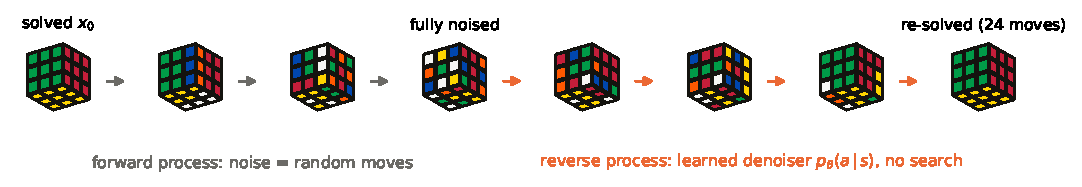
\includegraphics[width=\linewidth]{fig_teaser.pdf}
\captionof{figure}{Cube solving as denoising diffusion, end to end (real
states, trained model). \textbf{Left (gray):} the forward process noises the
solved state with random generator moves. \textbf{Right (orange):} the
learned reverse process---greedy rollout of the trained denoiser, no
search---removes the noise move by move; the 24-move solution shown is
replay-verified.}
\label{fig:teaser}
\vspace{0.5em}
\end{center}

\begin{abstract}
Solving the Rubik's Cube with learned heuristics is conventionally framed as
reinforcement learning: deep approximate value iteration (DAVI) learns a
cost-to-go function that guides search, as in DeepCubeA. We study an
alternative framing in which cube solving is \emph{discrete denoising
diffusion on a Cayley graph}: the forward (noising) process scrambles the
solved state with random generator moves under a linear depth schedule, and a
denoiser is trained by cross-entropy to predict the inverse of the last
scramble move---the exact analogue of $\epsilon$-prediction. Solving is
reverse-process sampling, optionally sharpened by beam search. The training
objective coincides with the self-supervised scramble-inversion objective of
Takano (2023); our contributions are the diffusion-process formalization, a
controlled matched-architecture, matched-hardware comparison against DAVI, and
an evaluation protocol with unusually strong guarantees: an exact
breadth-first-search oracle over the \emph{entire} $2{\times}2{\times}2$ group
(3{,}674{,}160 states) and mechanical replay verification of every claimed
solution. On a single consumer GPU, the denoising objective is $5\times$
cheaper per iteration than DAVI, reaches $99.989\%$ greedy (search-free) solve
rate over the full $2{\times}2{\times}2$ state space where DAVI reaches
$77.7\%$, and solves $1000/1000$ fully scrambled $3{\times}3{\times}3$ cubes
after $4.9$ hours of training versus $13.9$ hours for DAVI at the same solve
rate. Exact-oracle diagnostics reveal complementary error structure: the value
function degrades monotonically with distance-to-goal, while the denoiser's
per-move accuracy dips precisely where the scramble-length posterior is most
ambiguous. Ablations over the noise schedule and timestep conditioning support
the diffusion interpretation: a linear (uniform) schedule suffices, and
conditioning on the timestep is unnecessary because the group state determines
its own noise level. Code and full logs are released for reproducibility.
\end{abstract}

\section{Introduction}

Learning to solve the Rubik's Cube is a canonical benchmark for combining
neural function approximation with search in enormous discrete state spaces:
the $3{\times}3{\times}3$ cube group has $4.3\times10^{19}$ elements, a single
rewarding state, and no informative local structure that naive exploration can
exploit. A forward random walk essentially never finds the solved state, so
successful learned solvers manufacture supervision by working
\emph{backward} from the goal. DeepCubeA~\citep{agostinelli2019} does so with
deep approximate value iteration (DAVI): states are sampled by scrambling the
solved cube, a cost-to-go network is trained by one-step Bellman backups, and
solutions are extracted with value-guided search.

This paper studies a different, arguably simpler framing, proposed
independently by the first author from the mechanics of generative diffusion
models~\citep{sohldickstein2015,ho2020}: treat scrambling as the
\emph{forward noising process} of a diffusion model whose data distribution is
a point mass on the solved state. Random generator moves substitute for
Gaussian noise; the scramble depth is the diffusion timestep; a linear
schedule (uniform over depths) replaces the cosine schedule; and the reverse
process is a learned denoiser that, given a noised (scrambled) state, predicts
the move that undoes the most recent noise increment---the exact discrete
analogue of the $\epsilon$-prediction objective. Solving a cube is then
nothing but reverse-process sampling from the fully-noised regime, optionally
sharpened by beam search, which plays the role of a guided sampler.

The resulting training signal---predict the inverse of the last scramble
move---is not new: it is precisely the self-supervised objective of
\citet{takano2023}, which outperformed DeepCubeA on solution optimality at
matched search budgets. What is missing from the literature, and what this
paper provides, is threefold:

\begin{enumerate}
\item \textbf{A diffusion-process formalization} (\S\ref{sec:method}) of
scramble-inversion training on Cayley graphs, which yields testable
predictions: the denoising target is a posterior average over scramble
histories (\ie{} inherently noisy labels), timestep conditioning should be
redundant because a group element determines its own distance-to-goal, and
schedule shape should matter only through the marginal state distribution it
induces.
\item \textbf{A controlled comparison} (\S\ref{sec:results}) against DAVI with
matched backbone architecture, batch size, data budget-per-iteration,
optimizer, hardware, and evaluation protocol---isolating the training
\emph{objective} as the only variable. Prior comparisons (\eg{}
\citealp{takano2023} vs.\ \citealp{agostinelli2019}) confound objective,
architecture, and compute.
\item \textbf{An exact evaluation protocol} (\S\ref{sec:setup}): for the
$2{\times}2{\times}2$ cube we enumerate the entire reachable group
(3{,}674{,}160 states) by GPU breadth-first search, giving exact optimal
distances against which value estimates, per-move decisions, and solution
optimality are measured \emph{exhaustively} rather than on samples; and every
claimed solution, on either cube, is verified by replaying its move sequence
in the environment. To our knowledge no prior learned-solver evaluation
reports full-state-space solve rates.
\end{enumerate}

Our findings are summarized as follows. At matched per-sample cost the
denoising objective is ${\sim}12\times$ cheaper than a DAVI iteration in
forward passes (no $|A|$-way neighbor expansion for bootstrapped targets) and
${\sim}5\times$ faster in measured wall clock. On the full
$2{\times}2{\times}2$ group the denoiser's search-free greedy rollout solves
$99.989\%$ of all states (DAVI: $77.7\%$), and both methods reach $100\%$ with
beam search---the denoiser needing only width $32$. On the
$3{\times}3{\times}3$, the denoiser solves $1000/1000$ hundred-move scrambles
after $4.9$\,h of training ($34.9\%$ of them with no search at all), matching
DAVI's solve rate at $2.8\times$ less wall clock; at every beam width the
denoiser dominates the value function in solve rate per unit of test-time
compute (Figure~\ref{fig:width}). The price is solution length: the denoiser's
likelihood-guided beam yields solutions averaging $29.9$ moves against DAVI's
$22.95$ in each method's own best configuration, and the gap closes to
${\sim}0.4$ moves under an identical beam implementation. Exact-oracle
diagnostics and ablations (\S\ref{sec:ablations}) corroborate the diffusion
view, including a characteristic dip in per-move accuracy at intermediate
distances where the posterior over scramble histories is most ambiguous.

\section{Related Work}
\label{sec:related}

\paragraph{Learned Rubik's Cube solvers.}
DeepCube~\citep{mcaleer2019} introduced autodidactic iteration, and
DeepCubeA~\citep{agostinelli2019} refined it into DAVI: train
$V_\theta(s)\approx\dstar(s)$ on reverse scrambles via one-step lookahead
targets, then solve with batch-weighted A*. Non-learned solvers achieve
optimality with pattern databases~\citep{korf1997}; the cube's QTM diameter is
26~\citep{rokicki2014}. \citet{takano2023} trains a policy to predict the
scramble-inverting move and decodes with beam search, reporting shorter
solutions than DeepCubeA at matched node budgets, with far less training data.
Our training objective for the denoiser is the same as Takano's; we do not
claim it as a contribution. Unlike \citet{takano2023}, we hold architecture,
batch, hardware, and evaluation fixed across both objectives, add exact
full-group evaluation, and interpret the method through the diffusion lens
with supporting ablations.

\paragraph{Denoising diffusion.}
Diffusion models learn to invert a gradual noising
process~\citep{sohldickstein2015,ho2020,song2019}; discrete-state variants
replace Gaussian kernels with categorical transition
matrices~\citep{austin2021,hoogeboom2021}. Noise schedules are a central
design choice in the continuous setting~\citep{nichol2021}. Diffusion-style
iterative refinement has been applied to combinatorial optimization, \eg{}
DIFUSCO~\citep{sun2023}, which denoises solution \emph{encodings} for TSP/MIS.
Our setting differs structurally: the ``noise'' is exogenous group action on a
Cayley graph, the data distribution is a point mass (the solved state), and
the reverse process outputs \emph{actions} rather than solution encodings,
making the sampler itself the solver.

\section{Method}
\label{sec:method}

\subsection{Setup: the cube as a Cayley graph}

Let $G$ be the cube group with identity $e$ (the solved state) and let
$A=\{a_1,\dots,a_M\}$ be a symmetric set of generators (quarter turns;
$a\in A \Rightarrow a^{-1}\in A$). States are represented as sticker
colorings $s\in\{0,\dots,5\}^{S}$; each generator acts as a fixed permutation
of the $S$ sticker indices, so a batch of moves is a single \texttt{gather}.
We use the quarter-turn metric throughout. For the $3{\times}3{\times}3$,
$M{=}12$, $S{=}54$. For the $2{\times}2{\times}2$ we restrict to
$A=\{U^{\pm1},R^{\pm1},F^{\pm1}\}$ ($M{=}6$, $S{=}24$), which fixes the DLB
corner; the reachable set then has exactly $7!\cdot3^6 = 3{,}674{,}160$
elements with QTM diameter $14$, small enough to enumerate exactly
(\S\ref{sec:setup}). Let $\dstar(s)$ denote the exact distance to $e$ in the
Cayley graph $\Gamma(G,A)$.

\subsection{Forward process: scrambling as noise}

The forward process starts at the data distribution---a point mass
$q_0=\delta_e$ (``in the beginning, the cube is fully built'')---and applies
$t$ random generators:
\begin{equation}
s_0 = e,\qquad
a_k \sim \mathrm{Unif}\!\left(A\setminus\{a_{k-1}^{-1}\}\right),\qquad
s_k = a_k \cdot s_{k-1},\qquad k=1,\dots,t ,
\label{eq:forward}
\end{equation}
where excluding the immediate inverse removes the trivial 2-cycle (the
discrete analogue of using non-degenerate noise increments). The timestep is
drawn from a \emph{linear schedule} $t\sim\mathrm{Unif}\{1,\dots,K\}$ with
horizon $K$ ($K{=}18$ for the $2{\times}2{\times}2$, $K{=}30$ for the
$3{\times}3{\times}3$; both exceed the respective diameters). Unlike Gaussian
diffusion there is no signal-to-noise ratio to shape, so the cosine schedule
of \citet{nichol2021} has no analogue; the schedule matters only through the
marginal state distribution $q_t$ it induces, a claim we test in
\S\ref{sec:ablations}. As $t$ grows past the graph's mixing scale, $q_t$
approaches the uniform distribution on $G$---the fully-noised regime.
Figure~\ref{fig:forward} places this forward process in the diffusion lineage
visually: the same schedule semantics carry from the particle-density setting
of the original diffusion formulation through image DDPMs to the cube group,
with ``pure noise'' meaning, respectively, an isotropic Gaussian, a noise
image, and a uniformly random group element.

\begin{figure}[t]
\centering
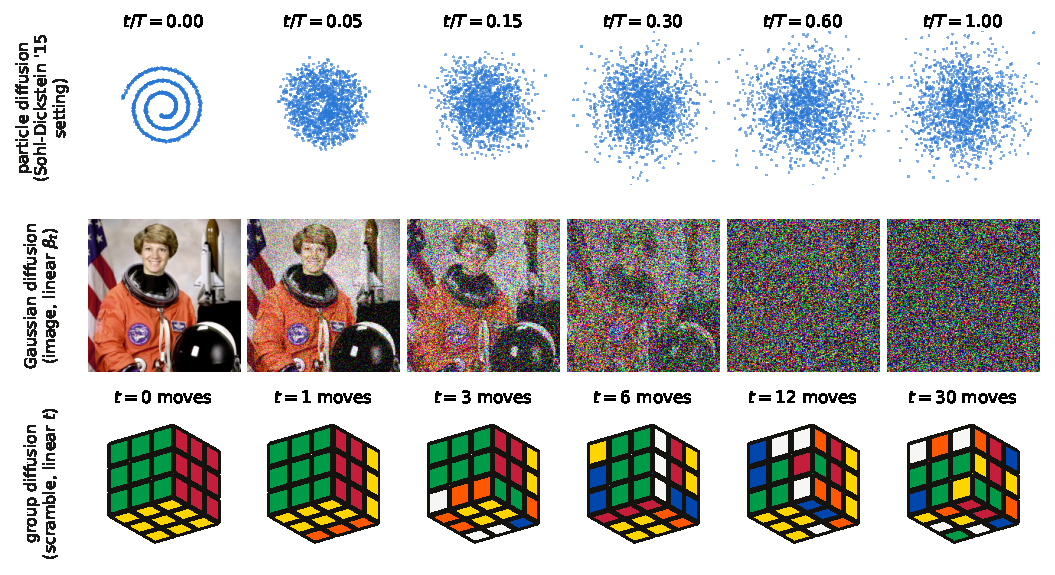
\includegraphics[width=\linewidth]{fig_forward_process.pdf}
\caption{One forward process, three state spaces, at matched noise levels
(left to right). \textbf{Top:} particle diffusion of a 2-D spiral density
into an isotropic Gaussian---the setting in which diffusion models were
introduced~\citep{sohldickstein2015} (our rendering). \textbf{Middle:}
Gaussian image diffusion under the linear DDPM
schedule~\citep{ho2020}, applied to a standard public-domain test photograph
(pixel-space noising, unrelated to the cube).
\textbf{Bottom:} the group forward process of this paper---the identical cube
after $t$ uniformly random generator moves (actual engine states). In all
three, a linear schedule interpolates between the data distribution and the
fully-noised regime; on the cube the ``noise'' is exogenous group action and
the fully-noised regime is a uniformly random state.}
\label{fig:forward}
\end{figure}

\subsection{Reverse process: noise prediction and sampling}

The denoiser $p_\theta(a\mid s)$ is trained to predict the inverse of the last
applied generator:
\begin{equation}
\mathcal{L}(\theta) \;=\;
\mathbb{E}_{t,\,a_{1:t}}\!\left[-\log p_\theta\!\left(a_t^{-1}\,\middle|\,s_t\right)\right],
\label{eq:loss}
\end{equation}
the categorical counterpart of $\epsilon$-prediction: the network observes a
noised sample and regresses the most recent noise increment. The Bayes-optimal
solution of Eq.~\eqref{eq:loss} is the posterior over last-move inverses given
the state,
\begin{equation}
p^{*}(a \mid s) \;\propto\; \textstyle\sum_{t=1}^{K}
\Pr\!\left[\,s_t = s,\; a_t = a^{-1}\,\right],
\label{eq:posterior}
\end{equation}
a \emph{posterior average over scramble histories}. Labels are therefore
inherently noisy---a walk that has already wandered back toward $e$ produces a
label pointing away from the goal---but the average correlates strongly with
descent on $\dstar$, and we quantify exactly how strongly in
\S\ref{sec:results} using the oracle. Two properties distinguish this from
continuous diffusion and motivate our design:

\textbf{No timestep conditioning.} In Gaussian diffusion the denoiser needs
$t$ because a given $x$ can occur at any noise level. On a Cayley graph the
state determines its own noise level: $\dstar(s)$ is a function of $s$, and
the set of distance-reducing generators $\arg\min_a \dstar(a\cdot s)$ does not
depend on how many steps produced $s$. We therefore drop $t$-conditioning and
validate this choice by ablation (\S\ref{sec:ablations}).

\textbf{No closed-form marginal, biased shell coverage.} Gaussian diffusion
reaches any noise level in one jump with the correct marginal by construction.
Here $q_t$ must be realized by walking, which is cheap ($t\le K$ gathers) but
\emph{biased}: random walks backtrack, so deep distance shells are reached far
less often than their share of the group. Both objectives inherit this bias;
we observe its signature in the error structure of both methods
(Figure~\ref{fig:errors}).

\textbf{Samplers.} Solving is reverse-process sampling from an arbitrarily
noised state. We use (i) \emph{greedy ancestral} decoding: iteratively apply
$\arg\max_a p_\theta(a\mid s)$ with the immediate backtrack masked, and (ii)
\emph{beam search} of width $W$ maximizing the cumulative log-likelihood
$\sum_i \log p_\theta(a_i \mid s_i)$---approximate MAP decoding of the reverse
trajectory, the discrete counterpart of a guided sampler. Search is an
optional sharpener, not a crutch: we report all results at $W{=}1$ as well.
Figure~\ref{fig:reverse} shows both reverse processes side by side---a small
DDPM we train on the classic spiral density reconstructing it from Gaussian
noise, and our trained denoiser's actual greedy rollout reconstructing the
solved cube from a 100-move scramble. The denoiser's confidence rises
monotonically as the state approaches the data manifold ($25\%\to97\%$ along
the trajectory shown), the discrete analogue of the sharpening posterior in
the final steps of Gaussian reverse diffusion.

\begin{figure}[t]
\centering
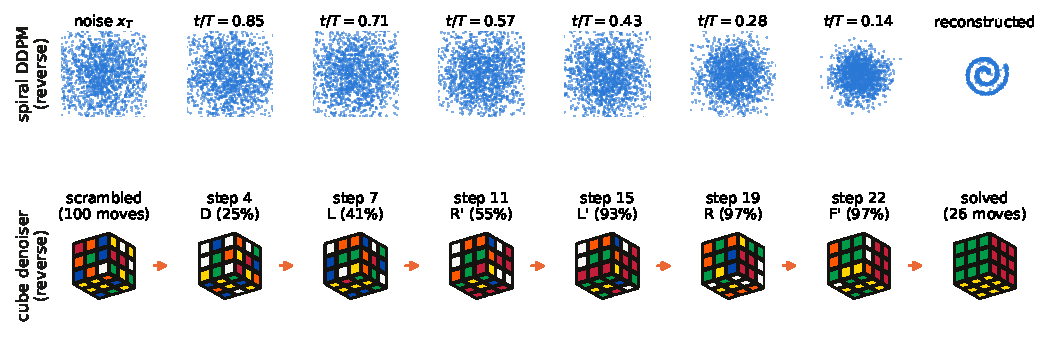
\includegraphics[width=\linewidth]{fig_reverse_process.pdf}
\caption{Reverse processes reconstruct the data from noise. \textbf{Top:} a
small DDPM trained here on the spiral density (the classic reconstruction
demonstration of the original diffusion paper~\citep{sohldickstein2015})
walks 1{,}600 particles from $\mathcal{N}(0,I)$ back onto the spiral. \textbf{Bottom:} the trained cube denoiser's
\emph{actual} greedy rollout (no search) on a 100-move scramble: each panel
shows the chosen move and its probability under $p_\theta$; the 26-move
solution is replay-verified. Confidence rises as noise is removed, in both
domains.}
\label{fig:reverse}
\end{figure}

\subsection{Baseline: deep approximate value iteration}

DAVI~\citep{agostinelli2019} trains $V_\theta(s)\approx\dstar(s)$ on the same
scramble distribution with bootstrapped one-step targets
$y(s) = 1 + \min_{a} V_{\bar\theta}(a\cdot s)$ (zero at $e$), where the target
network $\bar\theta$ is synced when the loss falls below a threshold. Each
iteration therefore costs $1{+}M$ forward passes per sample ($M$-way neighbor
expansion for the target plus the training pass) versus one for the denoiser.
At solve time the value function guides beam search by smallest predicted
cost-to-go. Backbone, batch size, optimizer, learning-rate schedule, scramble
distribution, and hardware are identical to the denoiser's
(Appendix~\ref{app:hyper}); the two methods differ only in output head
($1$ scalar vs.\ $M$ logits) and objective. Figure~\ref{fig:arch} shows the
shared architecture executing a real forward pass through both trained heads.

\begin{figure}[t]
\centering
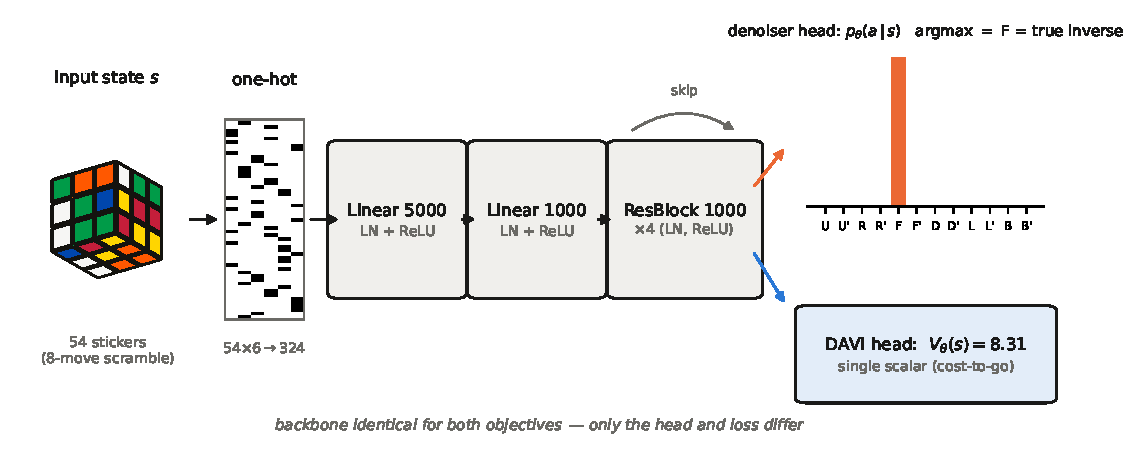
\includegraphics[width=\linewidth]{fig_architecture.pdf}
\caption{The shared architecture, shown on a \emph{real} forward pass through
both trained $3{\times}3{\times}3$ networks. A state eight scramble moves
from solved (left, actual engine state) is one-hot encoded and passed through
the common residual-MLP backbone. The trained denoiser head (top right,
actual output distribution) places nearly all probability on the true inverse
of the last scramble move; the trained DAVI head (bottom right) reads
$V_\theta(s)=8.31$ for this 8-move scramble. The two objectives share every
parameter except the final linear layer.}
\label{fig:arch}
\end{figure}

\section{Experimental Setup}
\label{sec:setup}

\paragraph{Vectorized environment.}
All experiments run on one consumer laptop GPU (NVIDIA RTX~5080 Laptop,
16.6\,GB). States are int8 tensors $[B,S]$; each generator is a precomputed
permutation; stepping $B$ cubes is one \texttt{gather} (measured
$0.25$--$0.5$ billion moves/s at $B{=}10^5$--$10^6$ even while training
occupies the GPU). Move tables are generated geometrically (rotating sticker
positions and normals, then re-matching), not hand-coded.

\paragraph{Engine and oracle validation.}
The engine passes group-theoretic identities (generator order $4$, inverse
consistency, sexy-move order $6$, $(RU)$ order $105$ on the
$3{\times}3{\times}3$, chirality checks). For the $2{\times}2{\times}2$, GPU
breadth-first search from $e$ enumerates the reachable set in $0.6$\,s,
reproducing the known group order $3{,}674{,}160$, QTM diameter $14$, and the
published distance distribution (\eg{} exactly $276$ states at depth $14$),
which pins the move tables exactly and yields an oracle table of
$\dstar$ for every state.

\paragraph{Verification protocol.}
A cube counts as solved only if replaying the emitted move sequence from the
scramble state in the environment lands exactly on $e$. Every number below
passed this check; no solver output is trusted.

\paragraph{Protocol.}
Both methods use residual MLP backbones with LayerNorm
(Appendix~\ref{app:hyper}): $1.7$M parameters for the $2{\times}2{\times}2$,
$14.7$M for the $3{\times}3{\times}3$, batch $10{,}000$, Adam,
$10\times$ LR decay at $80\%$ of iterations, bf16 autocast,
\texttt{torch.compile} for the $3{\times}3{\times}3$. DAVI trains for its
standard budget (40k iterations on the $2{\times}2{\times}2$; 250k on the
$3{\times}3{\times}3$); the denoiser trains for 40k and 500k respectively, and
we additionally report the denoiser at \emph{matched iterations} (250k) and
throughout \emph{matched wall clock}. $3{\times}3{\times}3$ test sets are
$1000$ fresh cubes scrambled with $100$ random moves (far beyond the QTM
diameter $26$); results are single-seed (see Limitations).

\section{Results}
\label{sec:results}

\subsection{The full $2{\times}2{\times}2$ group, exhaustively}

Table~\ref{tab:2x2} reports both solvers evaluated on \emph{all}
$3{,}674{,}160$ states. The denoiser trains in one quarter of the wall clock,
solves $99.989\%$ of the entire group with greedy rollout alone (DAVI:
$77.7\%$), and closes to $100\%$ with a width-$32$ beam; DAVI requires
escalating widths up to $32{,}768$ to solve its final holdout state. Greedy
solution lengths are near-optimal for the denoiser ($11.59$ vs.\ the exact
optimum $10.67$ averaged over its greedy-solved set).

\begin{table}[t]
\centering
\small
\begin{tabular}{lcc}
\toprule
& DAVI (value) & Denoising (ours) \\
\midrule
Parameters & 1.7M & 1.7M \\
Training iterations & 40{,}000 & 40{,}000 \\
Training wall clock & 26\,min & \textbf{6.5\,min} \\
Greedy solve rate, all 3{,}674{,}160 states & 77.67\% & \textbf{99.989\,\%} \\
\quad avg length (vs.\ exact optimal) & 15.05 (10.52) & \textbf{11.59} (10.67) \\
Beam-search solve rate (all states) & 100.000\% & 100.000\% \\
\quad max beam width needed & 32{,}768 & \textbf{32} \\
Full-sweep evaluation time & ${\sim}35$\,min & \textbf{${\sim}20$\,s} \\
\bottomrule
\end{tabular}
\caption{Exhaustive evaluation over the entire $2{\times}2{\times}2$ group
(URF generators). Every solution replay-verified. DAVI's value-guided and the
denoiser's likelihood-guided beams use their respective native scoring.}
\label{tab:2x2}
\end{table}

\paragraph{Exact error structure.}
Figure~\ref{fig:errors} uses the oracle to dissect both models. DAVI's value
error grows monotonically with $\dstar$ (MAE $4.1$ moves at $\dstar{=}14$):
bootstrapped values propagate outward from $e$ and the walk-induced training
distribution under-covers deep shells. The denoiser's per-move accuracy---the
probability that its argmax move strictly reduces $\dstar$---is instead
non-monotone: perfect near the goal \emph{and} at the diameter, with a dip to
$70$--$75\%$ at $\dstar\in\{10,11\}$. This is the signature predicted by the
posterior-averaging view (Eq.~\ref{eq:posterior}): at intermediate distances
the posterior over scramble histories passing through $s$ is maximally
ambiguous, so labels are noisiest; at the diameter, by contrast, almost every
neighbor of a depth-14 state has depth 13, so nearly any move is correct.

\begin{figure}[t]
\centering
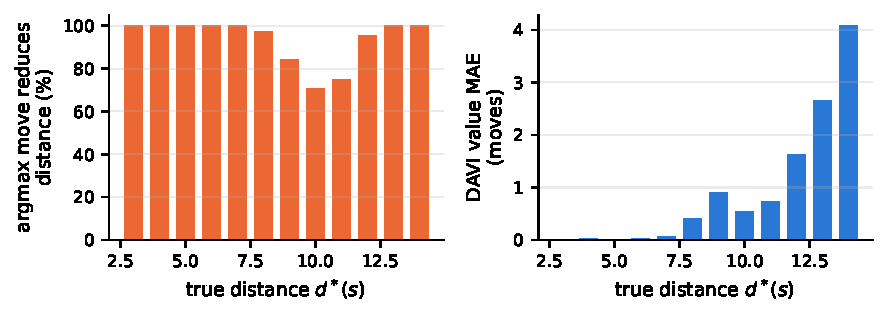
\includegraphics[width=0.86\linewidth]{fig_error_structure.pdf}
\caption{Exact-oracle error structure on the $2{\times}2{\times}2$
(100k uniform states). \textbf{Left:} probability that the denoiser's argmax
move strictly reduces true distance, by $\dstar$. \textbf{Right:} DAVI value
MAE by $\dstar$. The two objectives fail in complementary, mechanistically
interpretable ways.}
\label{fig:errors}
\end{figure}

\subsection{$3{\times}3{\times}3$: matched compute, full scrambles}

Table~\ref{tab:3x3} gives the headline comparison; Figure~\ref{fig:training}
shows greedy capability versus training wall clock. Both methods ultimately
solve $1000/1000$ fully scrambled cubes with width-2048 beams. The differences
are (i) \emph{training cost}---the denoiser reaches $100\%$ after $4.9$\,h
(and already matches DAVI's final solve rate at matched iterations, reached in
$2.4$\,h) versus $13.9$\,h for DAVI; (ii) \emph{search dependence}---the
denoiser solves $349/1000$ cubes with no search whatsoever, while DAVI's
greedy descent solves none (its value plateaus leave greedy trajectories
orbiting); and (iii) \emph{solution length}---DAVI's best configuration
produces solutions averaging $22.95$ moves (max $28$, near the QTM diameter
$26$) versus $29.88$ for the denoiser's likelihood-guided beam. Length is the
one axis on which the value function retains an advantage in its own solver
configuration; under an identical beam implementation the gap nearly vanishes
(below).

\begin{table}[t]
\centering
\small
\begin{tabular}{lccc}
\toprule
& DAVI (value) & \multicolumn{2}{c}{Denoising (ours)} \\
\cmidrule(lr){3-4}
& 250k iters & 250k iters (matched) & 500k iters \\
\midrule
Parameters & 14.7M & 14.7M & 14.7M \\
Wall clock & 13.9\,h & \textbf{2.4\,h} & 4.9\,h \\
Iterations/s (steady) & 5.8 & \textbf{28.7} & 28.7 \\
Solve rate (1000 cubes, beam 2048) & 100\% & 100\% & 100\% \\
Greedy-only solve rate & 0\% & 25.7\% & \textbf{34.9\%} \\
Avg solution length & \textbf{22.95} & 29.02 & 29.88 \\
Max solution length & \textbf{28} & 60 & 60 \\
Eval wall clock (1000 cubes) & 12.0\,min & \multicolumn{2}{c}{\textbf{${\sim}1$\,min}} \\
\bottomrule
\end{tabular}
\caption{$3{\times}3{\times}3$ on 1000 hundred-move scrambles, all solutions
replay-verified. Each method uses its native beam scoring (value vs.\
cumulative log-likelihood); see Figure~\ref{fig:width} for the
implementation-matched comparison.}
\label{tab:3x3}
\end{table}

\begin{figure}[t]
\centering
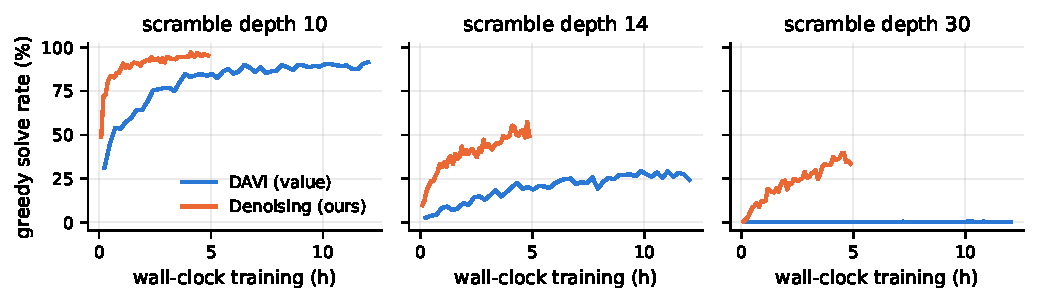
\includegraphics[width=\linewidth]{fig_training.pdf}
\caption{Greedy (search-free) solve rate versus training wall clock on the
$3{\times}3{\times}3$, by scramble depth (512 cubes per probe). The denoising
objective converts GPU-hours into search-free capability several times faster
than value iteration, and is the only method that lifts off at depth 30
within either budget.}
\label{fig:training}
\end{figure}

\subsection{Test-time compute scaling}

Figure~\ref{fig:width} holds the solver implementation fixed---the same
batched, deduplication-free beam for both methods---and sweeps the width. The
denoiser dominates at every width: at $W{=}512$ it solves $100\%$ of 200
scrambles in $4.1$\,s total, where the value net solves $26.5\%$ in
$102$\,s. Two subtleties deserve emphasis. First, solution lengths converge at
large widths ($23.75$ vs.\ $24.1$ at $W{=}2048$): the denoiser's longer
solutions in Table~\ref{tab:3x3} are a property of likelihood-guided decoding,
not of the learned representation. Second, DAVI is far more sensitive to
solver implementation: with a sequential beam that maintains a visited-set
(deduplicating revisits), DAVI recovers $100\%$ at $W{=}2048$
(Table~\ref{tab:3x3}), while the no-dedup beam above reaches only $59.5\%$.
Value-guided beams collapse onto plateaus of near-equal predicted cost unless
revisits are pruned; likelihood-guided beams diversify intrinsically because
path scores accumulate. We report both configurations for fairness.

\begin{figure}[t]
\centering
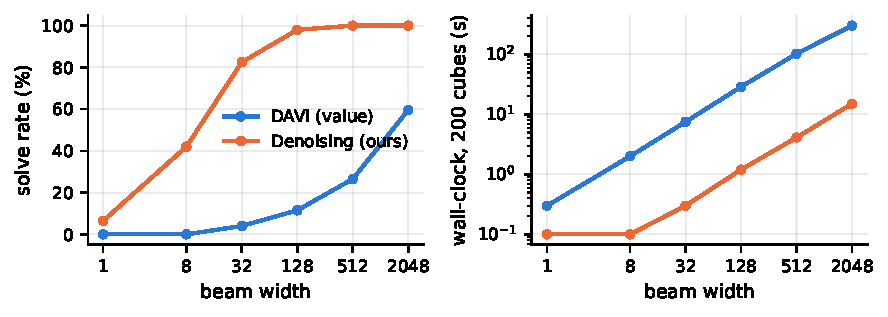
\includegraphics[width=0.86\linewidth]{fig_width_scan.pdf}
\caption{Test-time compute scaling on the $3{\times}3{\times}3$ (200
hundred-move scrambles; identical batched no-dedup beam for both methods).
\textbf{Left:} solve rate vs.\ beam width. \textbf{Right:} wall clock
(log scale). The denoiser dominates at every width and is
${\sim}20\times$ faster at equal width because it scores candidates with the
parent's forward pass rather than evaluating every child.}
\label{fig:width}
\end{figure}

\subsection{Ablations: schedule and timestep conditioning}
\label{sec:ablations}

Table~\ref{tab:ablations} ablates the two choices most closely tied to the
diffusion analogy, on the $2{\times}2{\times}2$ where the entire group can be
swept---so differences of hundredths of a percent are exact counts of failed
states, not sampling noise (though all variants are single training runs).
Figure~\ref{fig:schedules} makes the schedule semantics precise: in Gaussian
diffusion the schedule shapes the signal-to-noise curve $\bar\alpha_t$; on
the cube it shapes \emph{distance-shell coverage}, which we can measure
exactly with the oracle. Every walk-based schedule under-covers the deep
shells relative to their share of the group (at $\dstar{=}12$, which contains
$36.8\%$ of all states, the uniform walk spends $11.8\%$ of its budget, the
deep-biased walk $18.2\%$, and the shallow-biased walk only $6.7\%$---while
spending $24\%$ of its samples on trivial depth-1 states).

\begin{figure}[t]
\centering
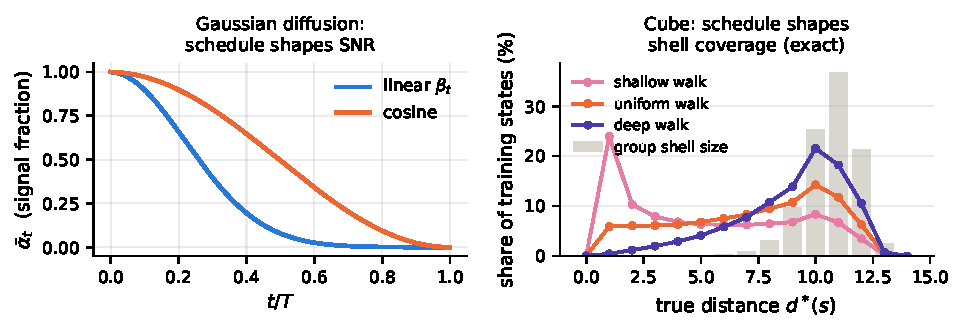
\includegraphics[width=0.88\linewidth]{fig_schedules.pdf}
\caption{What ``noise schedule'' means in each world. \textbf{Left:} in
Gaussian diffusion the linear and cosine~\citep{nichol2021} schedules shape
the signal fraction $\bar\alpha_t$---a knob with no analogue on a group,
where a move either happened or did not. \textbf{Right:} on the cube the
schedule acts only through the induced training distribution over true
distances, measured exactly here ($2{\times}10^6$ samples per schedule,
oracle-labeled, $2{\times}2{\times}2$, $K{=}18$). Gray bars are the exact
shell sizes of the group. All walk schedules under-cover deep shells; the
shallow-biased schedule starves them, matching its last-place coverage in
Table~\ref{tab:ablations}.}
\label{fig:schedules}
\end{figure}
\textbf{Schedule.} Every schedule reaches ${\ge}99.96\%$ search-free: the
objective is robust to schedule shape, as expected when the schedule matters
only through the induced state marginal. The ordering of the residuals is
nonetheless systematic and interpretable: shallow-biased sampling leaves
$3.5\times$ more unsolved states than the linear schedule (${\approx}1389$
vs.\ $402$), deep-biased sampling roughly halves them (${\approx}239$), and
per-move accuracy moves far less than coverage does. Deep-shell coverage, not
label quality, is the binding constraint. Setting the horizon to the exact
diameter ($K{=}14$) is marginally worse than over-noising ($K{=}18$) in
coverage; as in continuous diffusion, over-noising is cheap insurance (walk
depth over-estimates true distance, so $K$ beyond the diameter costs little).
\textbf{Timestep conditioning.} The $t$-conditioned variant is
\emph{not} better calibrated per move---its single-shot move accuracy is the
worst of all variants when queried at the fully-noised setting
($77.1\%$)---yet its annealed greedy rollout leaves the fewest unsolved states
(${\approx}107$). We read this as $t$-annealing acting as a mild decode-time
diversity mechanism (the policy is not a fixed function along the rollout, so
deterministic cycles are broken), not as evidence that the denoiser needs the
noise level: dropping $t$ entirely still solves $99.989\%$ with a strictly
simpler model. The state carries its own noise level; conditioning on $t$ is
optional, not necessary.

\begin{table}[t]
\centering
\small
\begin{tabular}{lcccc}
\toprule
Variant & Schedule & Greedy solve rate (all states) & ${\approx}$unsolved & Move quality \\
\midrule
Linear, $K{=}18$ (main) & uniform $1..18$ & 99.9891\% & 402 & 80.7\% \\
Linear, $K{=}14$ & uniform $1..14$ & 99.9865\% & 496 & \textbf{82.4\%} \\
Shallow-biased, $K{=}18$ & $d \propto$ small & 99.9622\% & 1389 & 79.3\% \\
Deep-biased, $K{=}18$ & $d \propto$ large & 99.9935\% & 239 & 81.6\% \\
$t$-conditioned, $K{=}18$ & uniform $1..18$ & \textbf{99.9971\%} & 107 & 77.1\% \\
\bottomrule
\end{tabular}
\caption{Noise-schedule and conditioning ablations on the
$2{\times}2{\times}2$: greedy (search-free) solve rate over all
$3{,}674{,}160$ states (with implied unsolved-state counts) and fraction of
argmax moves that strictly reduce exact distance (100k uniform states;
$t$-conditioned variant queried at $t{=}K$). 40k iterations each, single run
per variant. Shallow/deep bias: $d = \lceil K u^2\rceil$ / $d = \lceil K
\sqrt{u}\rceil$, $u\sim\mathrm{Unif}(0,1)$.}
\label{tab:ablations}
\end{table}

\subsection{Why does the denoiser need so much less search?}

DAVI must \emph{rank} neighbors by scalar value; adjacent values differ by at
most $1$, so ranking errors appear as soon as value MAE approaches $0.5$,
which happens by $\dstar{\approx}8$ (Figure~\ref{fig:errors}, right). Greedy
descent then cycles on plateaus, and beams without deduplication drown in
value ties. The denoiser sidesteps ranking through a direct
\emph{classification} of the descent direction: even with $19\%$ noisy labels
its argmax move makes progress at nearly every distance, so unguided rollouts
mostly reach the goal, and shallow beams absorb the residual label noise. In
diffusion terms: learning the score of the reverse kernel is easier than
learning the potential whose gradient it is.

\section{Discussion and Limitations}
\label{sec:limitations}

\textbf{What the analogy buys.} The diffusion framing is not decoration: it
predicted (i) that timestep conditioning is unnecessary, (ii) insensitivity
to schedule shape beyond induced coverage, (iii) the noisy-label structure of
the objective and where it should bite (the mid-distance dip), and (iv) that
over-noising ($K$ beyond the diameter) is safe. All four held empirically,
with one instructive nuance on (i): while the unconditioned denoiser loses
nothing in per-move accuracy, \emph{annealing} an optional $t$ input at decode
time breaks deterministic rollout cycles and further shrinks the (already
tiny) set of greedy failures---a decode-time effect, not a representation
requirement (\S\ref{sec:ablations}).

\textbf{What it does not buy.} There is no closed-form marginal: deep shells
are exponentially under-sampled by walks, a bias shared with DAVI and visible
in both error profiles. Likelihood-guided decoding optimizes plausibility, not
brevity---solution length is the one metric where the value function's own
solver wins ($22.95$ vs.\ $29.88$); combining both signals (denoiser proposals
scored by a value function) is an obvious hybrid we leave to future work.

\textbf{Scope.} Results are single-seed on one hardware platform; run-to-run
variance is not characterized, although the exhaustive $2{\times}2{\times}2$
sweep eliminates test-set noise entirely on that puzzle. We evaluate in QTM
only, on cubes only, and at a scale (14.7M parameters, $\le5\times10^9$
samples) far below DeepCubeA's original training; absolute solution-length
comparisons to published DeepCubeA numbers are therefore not meaningful. The
$2{\times}2{\times}2$ uses a restricted generator set (URF), standard but
different from the full-move convention. Solution lengths for the denoiser are
bounded by our rollout cap (60 moves).

\section{Reproducibility}

All code is a small self-contained repository (${\sim}1500$ lines: vectorized
environment with geometric move-table generation and group-identity tests, GPU
BFS oracle, both trainers, batched solvers with replay verification, and every
evaluation and figure script), released at
\url{https://github.com/aamirkhani/rubiks-diffusion}. All training logs and
evaluation JSON reports referenced here are included in the repository and are
regenerated by the released scripts; hyperparameters are listed in
Appendix~\ref{app:hyper}. Total compute for every experiment in this paper:
${\sim}22$ GPU-hours on one laptop GPU.

\bibliographystyle{plainnat}
\begin{thebibliography}{20}

\bibitem[Agostinelli et~al.(2019)]{agostinelli2019}
F.~Agostinelli, S.~McAleer, A.~Shmakov, and P.~Baldi.
\newblock Solving the {R}ubik's cube with deep reinforcement learning and search.
\newblock \emph{Nature Machine Intelligence}, 1(8):356--363, 2019.

\bibitem[Austin et~al.(2021)]{austin2021}
J.~Austin, D.~D. Johnson, J.~Ho, D.~Tarlow, and R.~van~den Berg.
\newblock Structured denoising diffusion models in discrete state-spaces.
\newblock In \emph{NeurIPS}, 2021.

\bibitem[Ho et~al.(2020)]{ho2020}
J.~Ho, A.~Jain, and P.~Abbeel.
\newblock Denoising diffusion probabilistic models.
\newblock In \emph{NeurIPS}, 2020.

\bibitem[Hoogeboom et~al.(2021)]{hoogeboom2021}
E.~Hoogeboom, D.~Nielsen, P.~Jaini, P.~Forr\'e, and M.~Welling.
\newblock Argmax flows and multinomial diffusion: Learning categorical distributions.
\newblock In \emph{NeurIPS}, 2021.

\bibitem[Korf(1997)]{korf1997}
R.~E. Korf.
\newblock Finding optimal solutions to {R}ubik's cube using pattern databases.
\newblock In \emph{AAAI}, 1997.

\bibitem[McAleer et~al.(2019)]{mcaleer2019}
S.~McAleer, F.~Agostinelli, A.~Shmakov, and P.~Baldi.
\newblock Solving the {R}ubik's cube with approximate policy iteration.
\newblock In \emph{ICLR}, 2019.

\bibitem[Nichol and Dhariwal(2021)]{nichol2021}
A.~Q. Nichol and P.~Dhariwal.
\newblock Improved denoising diffusion probabilistic models.
\newblock In \emph{ICML}, 2021.

\bibitem[Rokicki et~al.(2014)]{rokicki2014}
T.~Rokicki, H.~Kociemba, M.~Davidson, and J.~Dethridge.
\newblock The diameter of the {R}ubik's cube group is twenty.
\newblock \emph{SIAM Review}, 56(4):645--670, 2014.

\bibitem[Sohl-Dickstein et~al.(2015)]{sohldickstein2015}
J.~Sohl-Dickstein, E.~Weiss, N.~Maheswaranathan, and S.~Ganguli.
\newblock Deep unsupervised learning using nonequilibrium thermodynamics.
\newblock In \emph{ICML}, 2015.

\bibitem[Song and Ermon(2019)]{song2019}
Y.~Song and S.~Ermon.
\newblock Generative modeling by estimating gradients of the data distribution.
\newblock In \emph{NeurIPS}, 2019.

\bibitem[Sun and Yang(2023)]{sun2023}
Z.~Sun and Y.~Yang.
\newblock {DIFUSCO}: Graph-based diffusion solvers for combinatorial optimization.
\newblock In \emph{NeurIPS}, 2023.

\bibitem[Takano(2023)]{takano2023}
K.~Takano.
\newblock Self-supervision is all you need for solving {R}ubik's cube.
\newblock \emph{Transactions on Machine Learning Research}, 2023.

\end{thebibliography}

\appendix

\section{Hyperparameters and matched settings}
\label{app:hyper}

\begin{table}[h]
\centering
\small
\begin{tabular}{lcc}
\toprule
& $2{\times}2{\times}2$ & $3{\times}3{\times}3$ \\
\midrule
Backbone & \multicolumn{2}{c}{MLP: one-hot $\to$ $h_1$ $\to$ $h_2$ $\to$ residual blocks (LayerNorm, ReLU)} \\
$h_1$, $h_2$, blocks & 1024, 512, 2 & 5000, 1000, 4 \\
Output head (DAVI / denoiser) & scalar / 6 logits & scalar / 12 logits \\
Parameters & 1.7M & 14.7M \\
Batch size & 10{,}000 & 10{,}000 \\
Optimizer & \multicolumn{2}{c}{Adam, lr $10^{-3}$, $\times0.1$ at 80\% of iterations} \\
Precision & \multicolumn{2}{c}{bf16 autocast (+\texttt{torch.compile} on $3{\times}3{\times}3$)} \\
Scramble horizon $K$ & 18 (DAVI: 14 then 18) & 30 \\
Iterations (DAVI / denoiser) & 40k / 40k & 250k / 500k \\
DAVI target-net sync & \multicolumn{2}{c}{loss $<0.05$ checked every 100 iters; forced after 2000/5000} \\
Greedy rollout cap & 40 moves & 60 moves \\
Beam widths (main eval) & 32--32{,}768 & 2048 \\
Test scrambles & entire group & 1000 cubes, 100 moves, fixed seed \\
GPU & \multicolumn{2}{c}{NVIDIA RTX 5080 Laptop, 16.6\,GB} \\
\bottomrule
\end{tabular}
\caption{Matched configurations. The two methods differ only in output head
and training objective.}
\label{tab:hyper}
\end{table}

\section{Training-distribution statistics}

Measured over $10^6$ forward-process samples per puzzle: the scramble walk
terminates \emph{at} the solved state in $0.07\%$ ($2{\times}2{\times}2$) and
$0.01\%$ ($3{\times}3{\times}3$) of samples; at least one neighbor of the
sampled state is the solved state in $7.6\%$ and $3.4\%$ respectively. Under
the denoising objective every sample carries a defined label regardless; under
DAVI these near-goal encounters are the sole source of grounded (non-bootstrapped)
value signal. For contrast, a \emph{forward} random walk from a scrambled
$3{\times}3{\times}3$ state has $\Pr[\text{reach } e] \approx 2.3\times10^{-20}$
per step-sequence sample---the quantity that makes na\"ive exploration-based
RL infeasible on this domain.

\end{document}
